\section{Introduction}
\label{sec:intro}
\subsection{Preface}
\label{sec:intro.prefa}
\textit{PyCorrFit} emerged from my work in the Schwille Lab\footnote{\url{http://www.biochem.mpg.de/en/rd/schwille/}} at the Biotechnology Center of the TU Dresden in 2011/2012. Since then, the program has been further developed based on numerous input from FCS users, in particular Franziska Thomas, Grzesiek Chwastek, Janine Tittel, and Thomas Weidemann. The program source code is available at GitHub\footnote{\url{https://github.com/paulmueller/PyCorrFit}}. Please do not hesitate to sign up and add a feature request. If you you find a bug, please let us know via GitHub.\\

\noindent \textit{PyCorrFit} was written to simplify the work with experimentally obtained correlation curves. These can be processed independently (operating system, location, time). PyCorrFit supports commonly used file formats and enables users to allocate and organize their data in a simple way.\\

\noindent \textit{PyCorrFit} is free software: you can redistribute it and/or modify it
under the terms of the GNU General Public License as published 
by the Free Software Foundation, either version 2 of the License, 
or (at your option) any later version\footnote{\url{http://www.gnu.org/licenses/gpl.html}}.

\subsubsection*{What \textit{PyCorrFit} can do}
\begin{itemize}
\item Load correlation curves from numerous correlators
\item Process these curves
\item Fit a model function (many included) to an experimental curve
\item Import user defined models for fitting
\item Many batch processing features
\item Save/load entire \textit{PyCorrFit} sessions
\item \textbf{\LaTeX} support for data export
\end{itemize}

\subsubsection*{What \textit{PyCorrFit} is not}
\begin{itemize}
\item A multiple-$\tau$ correlator
\item A software to operate hardware correlators
\end{itemize}

\subsection{System prerequisites}
\label{sec:intro.prere}
\subsubsection{Hardware}
\label{sec:intro.prere.hardw}
This documentation addresses the processing of correlation curves with \textit{PyCorrFit} and was successfully used with the following setups:
\begin{itemize}
\item[1.]
     APD: Photon Counting Device from PerkinElmer Optoelectronics, Model: 	 \texttt{SPCM-CD3017}\\
     Correlator: Flex02-01D/C from correlator.com with the shipped software 	
	    		 \texttt{flex02-1dc.exe}.
\item[2.]
    APD: Photon Counting Device from PerkinElmer Optoelectronics\\
    Correlator: ALV-6000
\item[3.] LSM Confocor2 or Confocor3 setups from Zeiss, Germany.
\end{itemize}

\subsubsection{Software}
\label{sec:intro.prere.softw}
The latest version of \textit{PyCorrFit} can be obtained from the internet at \url{http://pycorrfit.craban.de}.
\begin{itemize}
\item \textbf{MacOS X.}
Binary files for MacOS X 10.9.5 and later are available from the download page.
\item \textbf{Windows.}
For Windows XP and later, stand-alone binary executables are available from the download page. 
\item \textbf{Ubuntu/Debian.}
PyCorrFit is available from the Debian repositories and can be installed via the operating systems packaging tool (e.g. \texttt{apt-get install pycorrfit}).
\item\textbf{PyPI.} To run \textit{PyCorrFit} on any other operating system, the installation of Python v.2.7 is required. \textit{PyCorrFit} is included in the Python package index (PyPI, \url{http://pypi.python.org/pypi/pip}) and can be installed via\footnote{See also the wiki article at \url{https://github.com/paulmueller/PyCorrFit/wiki/Installation_pip}}
\texttt{pip~install~pycorrfit$\!$[GUI]}.
\item \textbf{Sources.}
You can also directly download the source code at any developmental stage\footnote{See also the wiki article at \url{https://github.com/paulmueller/PyCorrFit/wiki/Running-from-source}}.
\end{itemize}


\vspace{1em}
\noindent \textbf{\LaTeX .} \textit{PyCorrFit} can save correlation curves as images using matplotlib. It is also possible to utilize \LaTeX to generate these plots. On Windows, installing MiKTeX  with ``automatic package download'' will enable this feature. On MacOS X, the MacTeX distribution can be used. On other systems, a latex distribution, Ghostscript, \texttt{dvipng} and the latex packages \texttt{texlive-latex-base} and \texttt{texlive-math-extra} need to be installed.


\subsection{Workflow}
\label{sec:intro.workf}

The following chapter introduces the general idea of how to start and accomplish a fitting project. FCS experiments produce different sets of experimental correlation functions which must be interpreted with appropriate physical models (\hyref{Chapter}{sec:theor}). Each correlation function refers to a single contiguous signal trace or ``run''. In \textit{PyCorrFit}, the user must assign a mathematical model function to each correlation function during the loading procedure. The assignment is irreversible in the sense that within an existing \textit{PyCorrFit} session it cannot be changed. This feature assures the stability of the batch processing routine for automated fitting of large data sets. Nevertheless, the fit of different models to the same data can be explored by loading the data twice or simply by creating two different sessions.

Let's briefly discuss a typical example: To determine the diffusion coefficient of a fluorescently labeled protein in free solution, one has to deal with two sets of autocorrelation data: measurements of a diffusion standard (e.g. free dye for which a diffusion coefficient has been published) to calibrate the detection volume and measurements of the protein sample. The protein sample may contain small amounts of slowly diffusing aggregates. While the calibration measurements can be fitted with a one-component diffusion model (T+3D), the protein sample displays two mobility states, monomers and aggregates, which are taken into account by a two-component diffusion model (T+3D+3D). With \textit{PyCorrFit} such a situation can be treated in three ways, having different pros and cons: 


\begin{enumerate}
\item Create separate sessions for each type of sample and assign different model functions.
\item Assign a one-component model to the dye measurements and a two-component model to the protein measurements when loading consecutively into the same session.
\item Assign a two-component model for all data and, when appropriate, manually inactivate one component by fixing its contribution to 0\%.
\end{enumerate}


The first approach is straightforward, however, it requires homogeneous diffusion behavior for each data set. The second strategy has the advantage that the dye and the protein curves, as well as the obtained parameters, can be visually compared during the fitting analysis within the same session. In this case, batch fitting is still possible because it discriminates data sets assigned to different models. In the third case, simultaneous batch fitting is also possible. However, for each dye measurement one has to eliminate the second, slow diffusion species manually, which might be laborious. Inactivating components by fixing parameters is nevertheless a common way to evaluate heterogeneous data sets, for example, a protein sample for which only a subgroup of curves requires a second diffusion component due to occasional appearance of aggregates. Such situations are frequently encountered in intracellular measurements. In conclusion, all three strategies or combinations thereof may be suitable. In any case, the user must decide on model functions beforehand, therefore it is advisable to group the data accordingly.

The fitting itself is usually explored with a representative data set. Here, the user has to decide on starting parameters, the range in which they should be varied, corrections like background, and other fitting options. Once the fit looks good, the chosen settings can be transferred at once to all other pages assigned to the same model using the \textit{Batch control} tool (\hyref{Section}{sec:menub.tools.batch}). After flipping through the data for visual inspection one may check the parameters across all pages in the \textit{Statistics view} tool and re-visit outliers (\hyref{Section}{sec:menub.tools.stati}). From there, the numerical fit values and example correlation functions can be exported.

\subsection{Graphical user interface (GUI)}
\label{sec:intro.graph}
\begin{figure}[h]
\centering
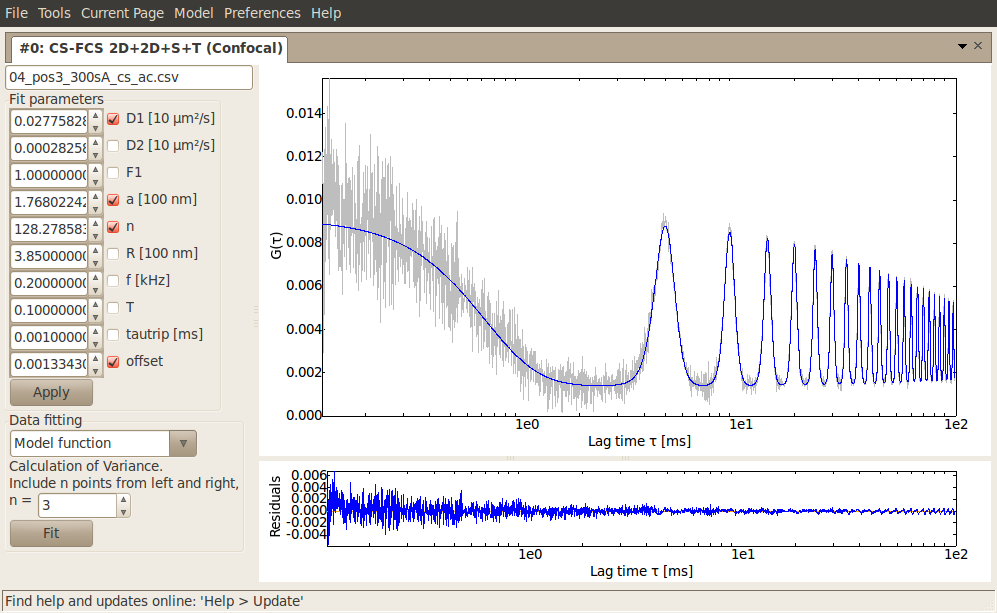
\includegraphics[width=\linewidth]{PyCorrFit_Screenshot_Main.png}
 \mycaption{user interface of PyCorrFit}{Confocal measurement of nanomolar Alexa488 in aqueous solution. To avoid after-pulsing, the autocorrelation curve was measured by cross-correlating signals from two detection channels using a 50 \% beamsplitter. Fitting reveals the average number of observed particles ($n \approx 6$) and their residence time in the detection volume ($\tau_{\rm diff} = \SI{28}{\mu s})$. \label{fig:mainwin} }
\end{figure}
Together with a system's terminal of the platform on which \textit{PyCorrFit} was installed (Windows, Linux, MacOS X), the \textit{main window} opens when starting the program. The window title bar contains the version of \textit{PyCorrFit} and, if a session was re-opened or saved, the name of the fitting session. A menu bar provides access to many supporting tools and additional information as thoroughly described in \hyref{Chapter}{sec:menub}. 

There are three gateways for experimental data into a pre-existing or a new \textit{PyCorrFit} session (\textit{File/Load data}, \textit{File/Open session}, and \textit{Current page/Import data}). When a session has been opened or correlation data have been loaded, each correlation curve is displayed on a separate page of a notebook. For quick identification of the active data set, a tab specifies the page number, the correlated channels (AC/CC), and the run number in cases where  multiple correlation runs are combined in a single file. When clicking a little triangle to the far-right, one can use a drop-down list of all page titles to directly access a particular data set. Alternatively, the pages can be toggled by tapping the arrow keys (left/right). There can be only one activated page for which the tab appears highlighted.

The active page displaying a correlation function is divided in two panels (\hyref{Figure}{fig:mainwin}). At the left hand side the page shows a pile of boxes containing values or fitting options associated with the current model and data set: 

\begin{itemize}
\item \textit{Data set} specifies the assigned model abbreviation in parentheses and shows a unique identifier for the correlation curve containing the file name, the number of the ``run'', and the data channel. This string is automatically assembled during the loading procedure (\hyref{Section}{sec:menub.filem.loadd}). However, during the session it can be manually edited, thereby allowing to re-name or flag certain data during the fitting analysis.
\item \textit{Model parameters} displays the values which determine the current shape of the assigned model function (\hyref{Chapter}{sec:theor}). Initially, starting values are loaded as they were defined in the model description (\hyref{Section}{sec:menub.filem.impor}). Little buttons allow a stepwise increase or decrease in units of 1/10\textsuperscript{th}. It is also possible to directly enter some numbers. A checkbox is used to set the parameter status to ``varied'' (checked) or ``fixed'' (unchecked) during the fitting. At the end, when saving the session, the current set of values together with their indicated names are stored in the *.yaml file (\hyref{Section}{sec:menub.filem.saves}). 
\item \textit{Amplitude corrections} applies additional rescaling to amplitude related parameters like the number of particles $n$ or amplitude fractions associated with different correlation times ($n_1$, $n_2$, etc.). Experimental values of non-correlated background intensity can be manually entered for each channel. In addition, the correlation curves can be normalized, to facilitate a visual comparison of the decay.
\item \textit{Fitting options} offers weighted fitting (a) and a choice for the fit algorithm (b).
\begin{itemize}
\item[\textbf{a)}] The underlying idea is that data points with higher accuracy should also have a higher impact on model parameters. To derive weights, \textit{PyCorrFit} calculates the variance of the difference between the actual data and a smooth, empiric representation of the curve for a certain neighbourhood. The number of neighbouring data points at each side ($j > 0$) can be set. For such a smooth representation a  spline function or the model function with the current parameter set can be used. The default number of knots for the spline function is 5. This number can be manually edited in the dropdown-selector. To view the spline function after each fit, \textit{Preferences/Verbose mode} has to be checked. If the current page is an average, then the standard deviation from the curves that were used to create the average can be used as weights.
\item[\textbf{b)}] Several fitting algorithms can be chosen. We recommend to use the Levenberg-Marquardt algorithm (b). For more information, see \hyref{Section}{sec:theor.alg}.
\end{itemize}
\end{itemize}
At the right hand side are two graphics windows. The dimensionless correlation functions $G(\tau)$ are plotted against the lag time ($\tau$) on a logarithmic scale. Below, a second window shows the residuals, the actual numerical difference between the correlation data and the model function. Fitting with appropriate models will scatter the residuals symmetrically around zero ($x$-axis). When weighted fitting was performed, the weighted residuals are shown. A good fit will not leave residuals systematically above or below the $x$-axis at any time scale.

The main window can be rescaled as a whole to improve data representation. In addition, to zoom in, one can drag a rectangle within the plot area; a double click then restores the initial scale. Experimental data points are linked by grey lines, the state of the model function is shown in blue. When a weighted fit was applied, the variance of the fit is calculated for each data point and displayed in cyan.

\section{The menu bar}
\label{sec:menub}
The menu bar organizes data management (File), data analysis (Tools), display of correlation functions (Current Page), numerical examples (Model), software settings (Preferences), and software metadata (Help).

\subsection{File menu}
\label{sec:menub.filem}
The File menu organizes the import of theoretical models, experimental correlation data, and opening and saving of entire \textit{PyCorrFit} fitting sessions. However, the numerical fit results are exported from the \textit{Statistics view} panel which can be found under \textit{Tools} (\hyref{Section}{sec:menub.tools.stati}).

\subsubsection{File / Import model}
\label{sec:menub.filem.impor}
Correlation data must be fitted to models describing the underlying physical processes which give rise to a particular time dependence and magnitude of the recorded signal fluctuations. Models are mathematical expressions containing parameters with physical meaning, like the molecular brightness or the dwell time through an illuminated volume. While the most commonly used standard functions are built-in, the user can define new expressions.
Some examples can be found at GitHub in the \textit{PyCorrFit} repository, e.g. circular scanning FCS \cite{Petrasek2008} (\hyref{Figure}{fig:csfcs}) or a combination of diffusion and directed flow \cite{Brinkmeier1999}. External model functions are discussed in detail in \hyref{Section}{sec:hacke.extmod}.


\subsubsection{File / Load data}
\label{sec:menub.filem.loadd}
\textit{Load data }is the first way to import multiple correlation data sets into a \textit{PyCorrFit} session. The supported file formats can be found in a drop-down list of supported file endings in the pop-up dialog \textit{Open data files}:

\begin{tabular}{l l}
 \rule{0pt}{3ex}  (1) All supported files & default \\

 \rule{0pt}{3ex} (2) ALV (*.ASC) & ALV Laser GmbH, Langen, Germany \\

 \rule{0pt}{3ex} (3) Correlator.com (*.SIN) & www.correlator.com, USA \\
 
 \rule{0pt}{3ex} (4) PicoQuant (*.pt3) & PicoQuant \\

 \rule{0pt}{3ex} (5) Zeiss ConfoCor3 (*.fcs) & AIM 4.2, ZEN 2010, Zeiss, Germany \\
 
 \rule{0pt}{3ex} (6) Matlab ‘Ries (*.mat) & EMBL Heidelberg, Germany \\

 \rule{0pt}{3ex} (7) PyCorrFit (*.csv) & Paul Müller, TU Dresden, Germany \\

 \rule{0pt}{3ex} (8) PyCorrFit session (*.pcfs) & Paul Müller, TU Dresden, Germany \\


 \rule{0pt}{3ex} (9) Zip file (*.zip) & Paul Müller, TU Dresden, Germany \\
\end{tabular}
\vspace{3ex}
\newline
While (2)-(5) are file formats associated with commercial hardware, (6) refers to a MATLAB based FCS evaluation software developed by Jonas Ries in the Schwille lab at TU Dresden, (7) is a text file containing comma-separated values (csv) generated by PyCorrFit via the command \textit{Current Page / Save data}. Zip-files are automatically decompressed and can be imported when matching one of the above mentioned formats. In particular loading of *.pcfs files (which are actually zip files) is a possibility to re-import correlation data from entire \textit{PyCorrFit} sessions. However, these data are treated as raw, which means that all fitting parameters and model assignments are lost.

During loading, the user is prompted to assign fit models in the \textit{Choose Models} dialogue window. There, curves are sorted according to channel (for example AC1, AC2, CC12, and CC21, as a typical outcome of a dual-color cross-correlation experiment). For each channel a fit model must be selected from the list (see \hyref{Section}{sec:menub.model}):

If a file format is not yet listed, the correlation data could be converted into a compatible text-file (*.csv) or bundles of *.csv files within a compressed archive *.zip. For reformatting correlation data, have a look at \hyref{Section}{sec:hacke.csv}.

\subsubsection{File / Open session}
\label{sec:menub.filem.opens}
This command is the second way to import data into PyCorrFit. In contrast to \textit{Load data}, it opens an entire fitting project, which was previously saved with \textit{PyCorrFit}. Session files are *.zip files named *.pcfs. These files contain all information to restore a session, including comments, model assigned correlation data, and the current state of parameters for each data set (\hyref{Section}{sec:menub.filem.saves}).

\subsubsection{File / Comment session}
\label{sec:menub.filem.comme}
This command opens a window to place text messages that can be used to annotate a fitting session.

\subsubsection{File / Clear session}
\label{sec:menub.filem.clear}
This command closes all pages. The user is prompted to save the current session.

\subsubsection{File / Save session}
\label{sec:menub.filem.saves}
In addition to display and fit individual curves, a strong feature of \textit{PyCorrFit} is to save an entire fitting project as a single session. Sessions allow the user to revisit and explore different models, fitting strategies, and data sets. Importantly the work can be saved at any stage.

The number of files bundled in a session varies depending on the number of data sets (pages), the number of used models, and what was done during the fitting. A detailed description can be found in the Readme.txt file attached to each session. For example, the numerical correlation and intensity data are saved separately as *.csv text files. However, in contrast to the \textit{Save data (*.csv)} command of the \textit{Current Page} menu, there are no metadata in the header, just tables containing the numerical values. In sessions, the fitting parameters are stored separately in the human-readable data serialization format *.yaml.

\subsubsection{File / Exit}
\label{sec:menub.filem.exit}
This command closes down \textit{PyCorrFit}. The user is prompted to save the session under the same or a different name.

\subsection{Tools menu}
\label{sec:menub.tools}
The \textit{Tools} menu provides access to a series of accessory panels which extent the capability of the main window. These accessory panels can stay open during the entire analysis. Open panels appear checked in the menu. Most operations can be executed across the entire data set with a single mouse click. 

\subsubsection{Tools / Data range}
\label{sec:menub.tools.datar}
This panel limits the range of lag times which are displayed in the main window panel. At the same time it defines the range of points which are used for fitting. For example, this feature can be applied to remove dominant after-pulsing of the avalanche photo diodes (APDs) which may interfere with Triplet blinking at short lag times. The user has the options to \textit{Apply} the channel settings only to the current page or he can \textit{Apply to all pages}. In contrast to \textit{Batch control}, this operation ignores whether the data are assigned to different models. 

Power user, who frequently load and remove data sets, may take advantage of a checkbox to fix the channel selection for all newly loaded data sets.

\subsubsection{Tools / Overlay curves}
\label{sec:menub.tools.overl}
This window displays the correlation data (not the fit curves) of all pages in a single plot. The curves can be discriminated by color. If only one curve is selected, it appears in red. Curves with ambiguous shape can easily be identified, selected, and removed by clicking \textit{Apply}. A warning dialogue lists the pages which will be kept.

Data representation is synchronized with the page display in the \textit{Main window}. For example, narrowing the range of lag times by \textit{Data range }is immediately updated in the \textit{Overlay curves }tool. Likewise, their normalization of the amplitudes to unity.

The other way round, some tools directly respond to the selections made in the \textit{Overlay curves} tool: \textit{Global fitting}, \textit{Average curves}, and \textit{Statistics view} allow to perform operations on an arbitrary selection of pages which can be specified by page number. Instead of manually typing their numbers, the curves may be selected within the \textit{Overlay curves} tool. The respective input fields are immediately updated.

The tool is closed by the button \textit{Cancel}. All the listed data sets will be kept. However, the selections transferred to the \textit{Global fitting}, \textit{Average curves}, and \textit{Statistics view} tools are kept as well.

\subsubsection{Tools / Batch control}
\label{sec:menub.tools.batch}
By default, the current page is taken as a reference to perform automated fitting. A batch is defined as the ensemble of correlation data sets (pages) assigned to the same model function within a session. A session can therefore have several batches, even for the same data. 

For fitting, it is crucial to carefully define the starting parameters, whether parameters should be fixed or varied, the range of values which make physically sense, and other options offered within the \textit{Main window}. By executing \textit{Apply to applicable pages}, these settings are transferred to all other pages assigned to the same fit model. Note that this includes the range of lag times (lag time channels) which may have been changed with the \textit{Data range }tool for individual pages.

The button \textit{Fit applicable pages} then performs fitting on all pages of the same batch. Alternatively, the user can define an external source of parameters as a reference, i.e. the first page of some \textit{Other session} (*.pcfs). However, this assumes a consistent assignment of model functions.

\subsubsection{Tools / Global fitting}
\label{sec:menub.tools.globa}
Global fitting is useful when experimental curves share the same values for certain physical parameters. For example, due to physical constraints in two-focus FCS both autocorrelation curves and  cross-correlation curves should adopt the same values for the diffusion time $\tau_\mathrm{diff}$ and the number of particles $n$. A global fit can be applied such that $n$ and $\tau_\mathrm{diff}$ are identical for all data sets. All curves are added to a single array. In contrast to fixing the shared parameters across a batch, in \textit{Global fitting} $\chi^2$  is minimized for all data sets simultaneously (see \hyref{Section}{sec:theor.nonle}). To perform \textit{Global fitting}, a subset of curves has to be selected by typing the numbers into the input field or by highlighting the pages via the \textit{Overlay curves} tool. 

\subsubsection{Tools / Average data}
\label{sec:menub.tools.avera}
Often in FCS, the measurement time at a particular spot is divided in several runs. This approach is taken when occasional, global intensity changes are superimposed on the molecular fluctuations of interest. Then the user has to sort out the bad runs. After fitting, one may want to re-combine the data to export a cleaned average correlation function. This can be done with the tool \textit{Average data}, for which a subset of curves has to be selected by typing the numbers into the input field or by highlighting the pages via the \textit{Overlay curves} tool. For averaging, there are constraints:


\begin{enumerate}
\item Since the correlation curves are averaged point by point this requires the same number of lag time channels. Runs of different length cannot be averaged.
\item The tool can only average data sets which are exclusively autocorrelation or cross-correlation.
\item The user can check a box to enforce the program to ask for data sets with the same model as the current page. This may help to avoid mistakes when selecting pages.
\end{enumerate}
The averaged curve is shown on a separate page. The new \textit{Filename/title} receives the entry \textit{Average [numbers of pages]}. The assigned model is by default the same as for the individual pages. However, while averaging, the user can choose a different model from a drop-down list. 

\subsubsection{Tools / Trace view}
\label{sec:menub.tools.trace}
FCS theory makes assumptions about the thermodynamic state of the system. Signal fluctuations can only be analyzed when the system is at equilibrium or at a sufficiently stable steady state. Global instabilities on the time scale of the measurement itself, e.g. photo-bleaching, have dramatic effect on the shape of the measured correlation curve. Therefore, it is common practice to check the correlated intensity trace for each curve. Trace view simply displays the signal trace for each correlation function. The window stays open during the session and can be used to revisit and flag ambiguous data sets.

\subsubsection{Tools / Statistics view}
\label{sec:menub.tools.stati}
The goal of a correlation analysis is to determine experimental parameter values with sufficient statistical significance. However, especially for large data sets, it can get quite laborious to check all of the individual values on each page. We designed the \textit{Statistics view} panel to review the state of parameters across the experimental batch (pages assigned to the same model) in a single plot, thereby facilitating to the identification of outliers.

The current page is taken as a reference for the type of model parameters which can be displayed. The user can choose different \textit{Plot parameters} from a drop-down list. A subset of pages within the batch can be explicitly defined by typing the page numbers into the input field or by highlighting in the \textit{Overlay curves} tool. Note that page numbers which refer to different models than the current page are ignored. 

The \textit{Statistics view} panel contains a separate \textit{Export} box, where parameters can be selected (checked) and saved as a comma separated text file (*.csv). Only selected page numbers are included.

\subsubsection{Tools / Page info}
\label{sec:menub.tools.pagei}
Page info is a most verbose summary of a data set. The panel \textit{Page info} is synchronized with the current page. The following fields are listed:


\begin{enumerate}
\item Version of \textit{PyCorrFit}
\item Field values from the main window (filename/title, model specifications, page number, type of correlation, normalizations)
\item Actual parameter values (as contained in the model function)
\item Supplementary parameters (intensity, counts per particle, duration, background correction, etc.)
\item Fitting related information (Chi-square, channel selection, varied fit parameters) .
\item Model doc string (\hyref{Section}{sec:menub.model})
\end{enumerate}
The content of Page info is saved as a header when exporting correlation functions via the command \textit{Current page / Save data (*.csv)} (\hyref{Section}{sec:menub.curre.saved}).

\subsubsection{Tools / Slider simulation}
\label{sec:menub.tools.slide}
This tool visualizes the impact of model parameters on the shape of the model function of a current page. Such insight may be useful to choose proper starting values for fitting or to develop new model functions. For example, in the case of two parameters that trade during the fitting one may explore to which extent a change in both values produces similar trends.

Two variables (A and B) have to be assigned from a drop-down list of parameters associated with the current model function. For each of these, the \textit{Slider simulation} panel shows initially the starting value (x) as a middle position of a certain range (from 0.1*x to 1.9*x). The accessible range can be manually edited and the actual value of the slider position is displayed at the right hand side of the panel. Dragging the slider to lower (left) or higher (right) values changes the entry in the box \textit{Model parameters} of the \textit{Main window} and accordingly the shape of the model function in the plot. By default the checkbox \textit{Vary A and B}\textit{ }is active meaning that both variables during \textit{Slider simulation} can be varied independently. 

In addition, the variables A and B can be linked by a mathematical relation. For this a mathematical operator can be selected from a small list and the option \textit{Fix relation} must be checked. Then, the variable B appears inactivated (greyed out) and the new variable combining values for A and B can be explored by dragging.

\subsection{Current Page}
\label{sec:menub.curre}
This menu compiles import and export operations referring exclusively to the active page in the main window. 

\subsubsection{Current Page / Import Data}
\label{sec:menub.curre.impor}
This command is the third way to import data into a pre-existing session. Single files containing correlation data can be imported as long as they have the right format (\hyref{Section}{sec:menub.filem.loadd}). In contrast to \textit{Load data} from the \textit{File} menu, the model assignment and the state of the parameters remains. The purpose of this command is to compare different data sets to the very same model function for a given set of parameters. After successful import, the previous correlation data of this page are lost.

To avoid this loss, one could first generate a new page via the menu \textit{Models} (\hyref{Section}{sec:menub.model}), select a model function and import data there. This is also a possibility to assign the very same data to different models within the same session.

\subsubsection{Current Page / Save data (*.csv)}
\label{sec:menub.curre.saved}
For the documentation with graphics software of choice, correlation curves can be exported as a comma-separated table. A saved \textit{PyCorrFit} text-file (*.csv) will contain a hashed header with metadata from the \textit{Page info} tool (\hyref{Section}{sec:menub.tools.pagei}), followed by the correlation and fitting values in tab-separated columns: \textit{Channel (tau [s])}, \textit{Experimental correlation}, \textit{Fitted correlation}, \textit{Residuals}, and \textit{Weights (fit)}. 

Below the columns, there are again 5 rows of hashed comments followed by the intensity data in two columns: \textit{Time [s]} and \textit{Intensity trace [kHz]}. Note that there are no assemblies of ``multiple runs'', since \textit{PyCorrFit} treats these as individual correlation functions. A *.csv file therefore contains only a single fitted correlation curve and one intensity trace for autocorrelation or two intensity traces for cross-correlation.

\subsubsection{Current Page / Save correlation as image}
\label{sec:menub.curre.savec}
The correlation curve can be exported as bitmap (e.g. *.png for quick documentation) or as a scalable vector graphic (e.g. *.pdf for post-processing in \textit{Adobe Illustrator} or \textit{Inkscape}). The plot contains a legend and fitting parameters. Note that the variable $\tau$ (= tau) cannot be displayed using Unicode with Windows. A \LaTeX formatted image can be exported when the option \textit{Use Latex} is checked in the \textit{Preferences} menu (\hyref{Section}{sec:menub.prefe}). Furthermore, if \textit{Preferences/Verbose mode} is checked, the plot can be edited before saving\footnote{The plots are generated with matplotlib, \url{http://matplotlib.org/}}. 

\subsubsection{Current Page / Save trace view as image}
\label{sec:menub.curre.savet}
An image of the trace can be exported in the same way as for the correlation curve (see above). 

\subsubsection{Current Page / Close page}
\label{sec:menub.curre.close}
Closes the page; the data set is removed from the session. The page numbers of all other pages remain the same. The command is equivalent with the closer (x) in the tab. 

\subsection{Models}
\label{sec:menub.model}
When choosing a model from the \textit{Models} menu, a new page opens and the model function is plotted according to the set of starting values for parameters as they were defined in the model description. The lists contains all of the implemented model functions, which can be selected during \textit{File / Load data}. The parameters can be manipulated to explore different shapes; the tool \textit{Slider simulation} can also be used. Via \textit{Current page / Import data}, the model may then be fitted to an experimental data set. Standard model functions for a confocal setup are (\hyref{Section}{sec:imple.confo}):

\begin{tabular}{l l}
%Confocal (Gaussian): 3D \ \ \ \ \ \ [Free diffusion in three dimensions]
\rule{0pt}{3ex} - Confocal (Gaussian): T+3D & Triplet blinking and 3D diffusion \\
\rule{0pt}{3ex} - Confocal (Gaussian): T+3D+3D & Triplet with two diffusive components \\
%Confocal (Gaussian): T+3D+3D+3D & [Triplet with three diffusive components]
%Confocal (Gaussian): 2D &  2D diffusion, e.g. in membranes \\
\rule{0pt}{3ex} - Confocal (Gaussian): T+2D &  Triplet blinking and 2D diffusion \\
\rule{0pt}{3ex} - Confocal (Gaussian): T+2D+2D & Triplet with two diffusive components \\
\rule{0pt}{3ex} - Confocal (Gaussian): T+3D+2D &  Triplet with mixed 3D and 2D diffusion \\
\rule{0pt}{3ex}
\end{tabular}

\noindent There is also a collection of models for FCS setups with TIR excitation (\hyref{Section}{sec:imple.tirfc}):

\begin{tabular}{l l}
\rule{0pt}{3ex} - TIR (Gaussian/Exp.): 3D & 3D diffusion \\
\rule{0pt}{3ex} - TIR (Gaussian/Exp.): T+3D+3D & Triplet with two diffusive components \\
\rule{0pt}{3ex} - TIR (Gaussian/Exp.): T+3D+2D & Triplet with mixed 3D and 2D diffusion \\
\rule{0pt}{3ex}
\end{tabular}

\noindent
In addition, there are may be user defined model functions which have been imported previously via \textit{File / Import model} (\hyref{Section}{sec:menub.filem.impor}).

\subsection{Preferences}
\label{sec:menub.prefe}
\paragraph*{Use Latex} If the user has a Tex distribution installed (e.g. MikTex for Windows), checking this option will generate \LaTeX formatted plots via the \textit{Current page / Save […] as image} commands.

\paragraph*{Verbose mode} If checked, this will cause the \textit{PyCorrFit} to display graphs that would be hidden otherwise. In weighted fitting with a spline, the spline function used for calculating the weights for each data points is displayed\footnote{For obvious reasons, such a plot is not generated when using the iteratively improved \textit{Model function} or the actual \textit{Average} correlation curve for weighted fitting.}. When saving the correlation curve as an image (\hyref{Section}{sec:menub.curre.savec}), the plot will be displayed instead of saved. If  ``Use Latex'' is checked, these plots will also be Latex-formatted. The advantage in displaying plots is the ability to zoom or rescale the plot from within \textit{PyCorrFit}.

\paragraph*{Show weights}
Checking this option will visualize the weights for each data point of the correlation function in the plot, as well as in the exported image. Note that the weights are always exported when using the \textit{Save data (*.csv)} command from the \textit{Current page} menu.

\subsection{Help}
\label{sec:menub.help}
\paragraph*{Documentation.}
This entry displays this documentation using the systems default PDF viewer.
\paragraph*{Wiki.}
This entry displays the wiki of \textit{PyCorrFit} on \textit{GitHub}. Everyone who registers with \textit{GitHub} will be able to make additions and modifications. The wiki is intended for end-users of \textit{PyCorrFit} to share protocols or to add other useful information.
\paragraph*{Update}
establishes a link to the \textit{GitHub} website to check for a new release; it also provides a few web links associated with \textit{PyCorrFit}
\paragraph*{Shell.}
This gives Shell-access to the functions of \textit{PyCorrFit}. It is particularly useful for trouble-shooting.
\paragraph*{Software.}
This lists the exact version of \textit{Python} and the corresponding modules with which \textit{PyCorrFit} is currently running.
\paragraph*{About.}
Information of the participating developers, the license, and documentation writers.


\section{Hacker's corner}
\label{sec:hacke}
\subsection{External model functions}
\label{sec:hacke.extmod}
\textit{PyCorrFit} supports the import of your own model functions. If your model function is not implemented, i.e. not available in the \textit{Models} menu, writing a short text file containing a model description is the easiest way to make \textit{PyCorrFit} work.
Some examples can be found at GitHub in the \textit{PyCorrFit} repository, e.g. circular scanning FCS \cite{Petrasek2008} (\hyref{Figure}{fig:csfcs}) or a combination of diffusion and directed flow \cite{Brinkmeier1999}. Model functions are imported as text files (*.txt) that must follow a certain format and syntax:
\begin{itemize}
\item \textbf{Encoding}: \textit{PyCorrFit} can interpret the standard Unicode character set. The model files have to be encoded in \textit{UTF-8}.
\item \textbf{Comments}: Lines starting with a hash (\texttt{\#}), empty lines, or lines containing only white space characters are ignored. The only exception is the first line starting with a hash followed by a white space and a short name of the model. This line is evaluated to complement the list of models in the dialogue\textit{ Choose }\textit{model}, when loading the data. Imported models are available from the menu \textit{Models/User}.
\item \textbf{Units}: \textit{PyCorrFit} works with internal units for:
\begin{itemize}
\item Time: \SI{1}{ms}
\item Distance: \SI{100}{nm}
\item Diffusion coefficient: \SI{10}{\mu m^2s^{-1}} 
\item Inverse time: \SI{1000}{s^{-1}} 
\item Inverse area: \SI{100}{\mu m^{-2}} 
\item Inverse volume: \SI{1000}{\mu m^{-3}} 
\end{itemize}
\item \textbf{Parameters:} To define a new model function, new parameters can be introduced. Parameters are defined by a sequence of strings separated by white spaces containing name, the dimension in angular brackets, the equal sign, and a starting value which appears in the main window for fitting. For example: \texttt{D [\SI{10}{\mu m^ 2 s^{-1}}] = 5.0}. User defined dimensions are only for display; thus mathematical expressions must correctly account for their conversion from internal units of \textit{PyCorrFit}. The parameter names contain only alphabetical (not numerical) characters. \texttt{G}, variables starting with \texttt{g}, as well as the numbers \texttt{e} and \texttt{pi} are already mapped and cannot be used freely.
\item \textbf{Placeholder:} When defining composite mathematical expressions for correlation functions, one can use place-holders. Place-holders start with a lower-case ‘g’. For example, the standard, Gaussian 3D diffusion in free solution may be written as

\begin{itemize}
\item \texttt{gTrp = 1+ T/(1-T)*exp(-tau/tautrip)}
\item \texttt{gTwoD = 1/(1+tau/taudiff)}
\item \texttt{gThrD = 1/sqrt(1+tau/(taudiff*S**2))}
\end{itemize}
\end{itemize}
The individual parts are then combined in the last line of the *.txt file, where the correlation function is defined starting with upper-case ’G’:

\begin{equation}
\texttt{G = 1/n * gTrp * gTwoD * gThrD} \notag
\end{equation}
For reference of mathematical operators, check for example \href{http://www.tutorialspoint.com/python/python_basic_operators.htm}{www.tutorialspoint.com / python / python\_basic\_operators.htm}. To illustrate a more complex example, a model function for circular scanning FCS is shown in \hyref{Figure}{fig:csfcs}. 
External models will be imported with internal model function IDs starting at $7000$. Models are checked upon import by the Python module sympy. If the import fails, there is most likely syntax error in the model file. 
\begin{figure}
% for case sensitiver Verbatim, we need the package fancyvrb
\begin{Verbatim}[frame = single]
# CS-FCS T+2D+2D+S (Confocal)

# Circular Scanning FCS model function for two 2D-diffusing species
# including triplet component.

## Definition of parameters:
# First, the parameters and their starting values for the model function
# need to be defined. If the parameter has a unit of measurement, then it 
# may be added separated by a white space before the "=" sign. The starting
# value should be a floating point number. Floating point abbreviations 
# like "1e-3" instead of "0.001" may be used.

# Diffusion coefficient of first component
D1 [10µm²/s] = 200.0
# Diffusion coefficient of second component
D2 [10µm²/s] = 20.0
# Fraction of species one
F1 = 1.0
# Half waist of the lateral detection area (w0 = 2*a)
a [100nm] = 1.0
# Particle number
n = 5.0
# Scan radius
R [100nm] = 3.850
# Frequency
f [kHz] = .2
# Triplet fraction
T = 0.1
# Triplet time
tautrip [ms] = 0.001
offset = 0.00001

# The user may wish to substitute certain parts of the correlation function
# with other values to keep the formula simple. This can be done by using 
# the prefix "g". All common mathematical functions, such as "sqrt()" or 
# "exp()" may be used. For convenience, "pi" and "e" are available as well.

gTriplet = 1. + T/(1-T)*exp(-tau/tautrip)
gScan1 = exp(-(R*sin(pi*f*tau))**2/(a**2+D1*tau))
gScan2 = exp(-(R*sin(pi*f*tau))**2/(a**2+D2*tau))
gTwoD1 = F1/(1.+D1*tau/a**2)
gTwoD2 = (1-F1)/(1.+D2*tau/a**2)

# The final line with the correlation function should start with a "G"
# before the "=" sign.

G = offset +  1./n * (gTwoD1 * gScan1 + gTwoD2 * gScan2) * gTriplet
\end{Verbatim}
\mycaption{user defined model function for PyCorrFit}{The working example shows a model function for circular scanning FCS (see also its appearance in the \textit{Main window} \hyref{Figure}{fig:csfcsplot} \label{fig:csfcs}}
\end{figure}

\subsection{Internal model functions}
Alternatively, new models can be implemented by programming of the models module of \textit{PyCorrFit}. First, edit the code for \texttt{\_\_init\_\_.py} and then add the script containing the model function. There is no Tutorial yet, but the implemented model files are self-explanatory. If you need help creating a new internal model function and/or want to publish it with \textit{PyCorrFit}, do not hesitate to contact an active developer by creating a new issue on GitHub.

\subsection{Correlation curve file format}
\label{sec:hacke.csv}
PyCorrFit can read correlation data from many file formats.
If a file format is not yet listed, the correlation data could be converted into a compatible text-file (*.csv) or bundles of *.csv files within a compressed *.zip archive. For reformatting the following requirements must be fulfilled:

\begin{itemize}
\item \textbf{Encoding}: \textit{PyCorrFit} uses the standard Unicode character set (UTF-8). However, since no special characters are needed to save experimental data, other encodings may also work. New line characters are \texttt{{\textbackslash}r{\textbackslash}n} (Windows).
\item \textbf{Comments}: Lines starting with a hash (\texttt{\#}), empty lines, or lines containing only white space characters are ignored. Exceptions are the keywords listed below.
\item \textbf{Units}: PyCorrFit works with units/values for:

\begin{itemize}
\item Time: \SI{1}{ms}
\item Intensity: \SI{1}{kHz}
\item Amplitude offset: $G(0) = 0$ (not 1)
\end{itemize}
\item \textbf{Keywords:}\footnote{Keywords are case-insensitive.} \textit{PyCorrFit} reads the first two columns containing numerical values. The first table (non-hashed) is recognized as the correlation data containing the lag times in the first and the correlation data in the second column. (In case the *.csv file has been generated with \textit{PyCorrFit} up to three additional columns containing the fit function are ignored). The table ends, when the keyword \texttt{\# BEGIN TRACE} appears. Below this line the time and the signal values should be contained in the first two columns. If cross-correlation data have to be imported a second trace can be entered after the keyword \texttt{\# BEGIN SECOND TRACE}.
\item \textbf{Tags:}\footnote{Tags are case-insensitive.} Channel information can be entered using defined syntax in a header. The keyword 
\begin{center}
\vspace{-1em}
 \texttt{\# Type AC/CC Autocorrelation}
\vspace{-1em}
\end{center}
  assigns the tag \texttt{AC} and the keyword
\begin{center}
\vspace{-1em}
  {\texttt{\# Type AC/CC Crosscorrelation}}
\vspace{-1em}
\end{center}
 assigns the tag \texttt{CC} to the correlation curve. These strings are consistently displayed in the user interface of the respective data page in \textit{PyCorrFit}. If no data type is specified, autocorrelation is assumed. Tags may be specified with additional information like channel numbers, e.g. 
\begin{center}
\vspace{-1em}
 \texttt{\# Type AC/CC Autocorrelation \_01}.
\vspace{-1em}
\end{center}
In this case the tag \texttt{AC\_01} is generated. This feature is useful to keep track of the type of curve during the fitting and when post-processing the numerical fit results.
\end{itemize}

\subsection{New file format}
Alternatively, new file formats can be implemented by programming of the readfiles module of \textit{PyCorrFit}. First, edit the code for \texttt{\_\_init\_\_.py} and then add the script \texttt{read\_FileFormat.py}.
There is no Tutorial yet, but the implemented scripts are self-explanatory. If you need help implementing a new file format and/or want to publish it with \textit{PyCorrFit}, do not hesitate to contact an active developer by creating a new issue on GitHub.

\section{Theoretical background}
\label{sec:theor}
In the first place, \textit{PyCorrFit} was designed to evaluate FCS data, therefore we focus on fluorescence. However, the correlation theory could be applied to any other stochastic signal.

\subsection{How FCS works}
\label{sec:theor.howfc}

FCS is a method to determine molecular properties of stochastically moving fluorescent molecules in solutions \cite{Elson1974,Magde1974,Magde1978}. The solution may be a liquid volume (3D) or a lipid membrane (2D) \cite{Widengren1998,Korlach1999,Schwille1999}. The diffusion may be free or anomalous due to barriers or obstacles \cite{Wachsmuth2000,Weiss2003}. The size of the diffusing particles range from synthetic dyes (\SI{800}{Da}) to large complexes or aggregates of labelled macromolecules (several MDa). Particles which differ in size or emission behaviour can be discriminated. Therefore FCS is a powerful tool to study molecular recognition \cite{Bacia2006,Kim2007}.

The measurement principle is to illuminate a small open volume within solutions of fluorescent molecules and to detect their molecular transits with a sub-microsecond time resolution by sensitive optics. The stochastic movements and other processes affecting fluorescence emission generate a fluctuating signal. The typical time pattern of these fluctuations can be revealed by a correlation analysis. The shape and time range of the decaying correlation function is defined by the exact geometry of the FCS detection volume in conjunction with the properties of the molecular system at hand. To derive hard numbers, the system must be parametrized as a theoretical model. Once the geometry of the detection volume is characterized, parameters can be determined by comparing the model function with experimental data (mathematical fitting, \hyref{Figure}{fig:mainwin}).

\subsection{Framework for a single type of fluorescent dye}
\label{sec:theor.frame}
The following equations are described in many papers in different ways. Here we follow the notation of one of us \cite{Weidemann2009}. Fluorescence signals are a result of absorption and emission of photons by a fluorophore. Under experimental conditions, the signal depends on the time dependent distribution of fluorescent particles in the sample volume $c(\vec{r},t)$ and the normalized instrumental detection efficiency $W(\vec{r})$. The total intensity, signal $S(t)$, is the sum of all photons emitted from fluorophores at different positions within the detection volume:
	\begin{equation}
	\label{eq1}
	S(t) = q \int W(\vec{r})  c(\vec{r},t) \,dV
	\end{equation}
The factor $q$ combines all the photo-physical quantities associated with fluorescence emission like absorption cross section, quantum yield, and the peak intensity of excitation (laser power). In the following, time averages of observables are indicated by angular brackets. We apply the ergodic theorem (see below).
	\begin{equation}
	\label{eq2}
	\langle S(t) \rangle = \lim_{t\to\ \infty} \int S(t) \,dt = q \int W(\vec{r})  c \,dV = qn
	\end{equation}
\hyref{Equation}{eq2} reveals that $q$ is the instrument dependent molecular brightness (kHz/particle), i.e. the average signal divided by the average number of particles $n$ observed within the effective detection volume $V_{\rm eff} = \int W(\vec{r})  \,dV$. During FCS measurements the detected signal is correlated by computing a normalized autocorrelation function: 
	\begin{equation}
	\label{eq3}
	G(\tau) = \frac{\langle S(t) \cdot S(t+\tau)\rangle}{\langle S(t) \rangle^2}-1 = \frac{\langle \delta S(t) \cdot \delta S(t+\tau)\rangle}{\langle S(t) \rangle^2} = \frac{g(\tau)}{\langle S(t) \rangle^2}
	\end{equation}
Here, $\tau$ denotes the lag time used for correlation and $\delta S(t) = S(t)-\langle S \rangle$ the amplitude of the signal fluctuation for a given time point. \hyref{Equation}{eq3} defines a function with a finite intercept decaying to zero, whereas $g(\tau)$, the non-normalized correlation function, decays to a finite value $\langle S \rangle^{-2}$. To visualize correlation times, the functions $G(\tau)$ are typically plotted against $\log(\tau)$ (\hyref{Figure}{fig:mainwin}).

A general way to derive theoretical model functions is to evaluate \hyref{Equation}{eq3} with explicit expressions describing the instrumental detection efficiency $W(\vec{r})$ and the molecular dynamics governing the local fluorophore concentrations $c(\vec{r},t)$. For example, free diffusion of the molecules can be described by the so-called diffusion propagator.
	\begin{equation}
	\label{eq4}
	P_\mathrm{d} \left( \vec{r} \,' | \vec{r},\tau \right) = \frac{1}{\left( 4 \pi D_t \tau \right) ^{3/2}} \exp \left[ - \frac{\left| \vec{r} \,' -\vec{r} \, \right|} {4D_t \tau} \right]
	\end{equation}
The propagator $P_\mathrm{d} \left( \vec{r} \,' | \vec{r},\tau \right)$ is the conditional probability of a particle with diffusion coefficient $D_t$ to move from $\vec{r}$ to $\vec{r \,'}$ within a time period $\tau$. 
The probability to find a particle inside the volume $d^3r$ is simply the ratio of  volumes $d^3r/V$.
 Such a diffusion propagator leads to a Gaussian shaped probability distribution spreading in time when the molecules successively roam the sample volume $V$.
Assuming that the time average and the ensemble average are equivalent (ergodic theorem), the average signal of a single particle is its molecular brightness $q$ normalized to its contribution to the entire volume, because the integral over the detection efficiency function is exactly the effective measurement volume $V_\mathrm{eff}$.
	\begin{equation}
	\label{eq5}
	\langle s(t) \rangle = q \frac{\int W(\vec{r}) \,dV}{V} = \frac{V_\mathrm{eff}}{V} q
	\end{equation}
Accordingly, we can express the average product of two signals separated by $\tau$ as
	\begin{equation}
	\label{eq6}
	\langle s(t) \cdot s(t + \tau) \rangle = \frac{q^2}{V}\iint W(\vec{r}) P_\mathrm{d} \left( \vec{r} \,' | \vec{r},\tau \right) W(\vec{r} \,') dVdV'
	\end{equation}
With the definition of the signal $S(t)$ and its average $\langle S(t) \rangle$
\begin{align}
S(t) &= \Sigma_{k=1}^n s_k(t) \\
\langle S(t) \rangle &= \Sigma_{k=1}^n \langle s_k(t) \rangle := N \langle s(t) \rangle
\end{align}
- where $N$ is the total number of particles in the sample volume $V$ - we can reduce $G(\tau)$ to the sum of individual molecular contributions
	\begin{align}
	G(\tau) = \frac{\langle S(t) \cdot S(t+\tau)\rangle}{\langle S(t) \rangle^2}-1 
	 =& \frac{\overbrace{N \langle s(t) \cdot s(t+\tau)\rangle}^{\mbox{\small same particles}} +\overbrace{N(N-1) \langle s(t) \rangle^2}^{\mbox{\small different particles}}}{N^2 \langle s(t) \rangle^2}-1  \notag \\
	\approx & \frac{\langle s(t) \cdot s(t+\tau)\rangle}{N \langle s(t) \rangle^2} \label{eq7} 
	\end{align}
Inserting \hyref{Equation}{eq5} and \hyref{Equation}{eq6} yields
	\begin{equation}
	\label{eq8}
	G(\tau) = \frac{V}{N} \frac{\iint W(\vec{r}) P_\mathrm{d} \left( \vec{r} \,' | \vec{r},\tau \right) W(\vec{r} \,') dVdV'}{\left( \int W(\vec{r}) \,dV \right)^2}
	\end{equation}
Note that the molecular brightness $q$ cancels; when considering multiple species with different $q$, this is no longer the case.
Solving these integrals for the confocal detection scheme yields a relatively simple equation containing the diffusion coefficient $D_t$ (molecular property) and the $1/e^2$ decay lengths $w_0$ and $z_0$ capturing the dimension of the Gaussian detection volume transversal and parallel to the optical axis, respectively (instrumental properties).
	\begin{equation}
	\label{eq9}
	G(\tau) = \frac{1}{n} \left(1+\frac{4 D_t \tau}{w_0^2} \right) ^{-1} \left(1+\frac{4D_t \tau}{z_0^2} \right)^{-1/2}
	\end{equation}
The inverse intercept $(G(0))^{-1}$ is proportional to the total concentration of oberved particles $C = N/V =  n/V_{\rm eff} = n/ (\pi^{3/2}w_0^2z_0)$. It is common to define the diffusion time $\tau_{\rm diff} = {w_0}^2/4D_t$ and the structural parameter $\textit{SP}=z_0^2/w_0^2$ as a measure of the elongated detection volume. Replacement finally yields the well known autocorrelation function for 3D diffusion in a confocal setup (Model ID 6012)
	\begin{equation}
	\label{eq10}
	G(\tau) \stackrel{\rm def}{=} G^{\rm D}(\tau) = \frac{1}{n} \overbrace{ \left(1+\frac{\tau}{\tau_{\rm {diff}}} \right) ^{-1}}^{\rm 2D} \overbrace{ \left(1+\frac{\tau}{\textit{SP}^2 \, \tau_{\rm {diff}}} \right)^{-1/2}}^{\rm 3D}
	\end{equation}
For confocal FCS, both the detection volume $W(\vec{r})$ and the propagator for free diffusion $P_\mathrm{d}$ are described by exponentials (Gaussian functions). Therefore, spatial relationships can be factorized for each dimension $xyz$. As a result, \hyref{Equation}{eq10} can be written as a combination of transversal (2D) and longitudinal (3D) diffusion.

\subsection{Autocorrelation of multiple species}
\label{sec:theor.autoc}
Very often in FCS, one observes more than one dynamic property. Besides diffusion driven number fluctuations, a fluorophore usually shows some kind of inherent blinking, due to triplet state transitions (organic dyes) or protonation dependent quenching (GFPs) \cite{Widengren1995}.
	\begin{equation}
	\label{eq11}
	G(\tau) \stackrel{\rm def}{=} G^{\rm T}(\tau) G^{\rm D}(\tau) = \left( 1+ \frac{T}{1-T} \exp\left[-\frac{\tau}{\tau_{\rm trp}} \right] \right)G^{\rm D}(\tau)
	\end{equation}
Blinking increases the correlation amplitude $G(0)$ by the triplet fraction $1/(1-T)$. Accordingly, the average number of observed particles is decreased $n = (1-T)/G(0)$. In case of GFP blinking, two different blinking times have been described and the rate equations can get quite complicated.
Besides photo-physics, the solution may contain mixtures of fluorescent particles with different dynamic properties, e.g. different mobility states or potential for transient binding. Such mixtures show several correlation times in the correlation curve. \hyref{Equation}{eq11} can be derived by considering the correlation functions of an ensemble, which can be built up by the contribution of $n$ single molecules in the sample volume:
	\begin{equation}
	\label{eq12}
	G(\tau) = \frac{g(\tau)}{\langle S(t) \rangle^2} = \frac{\sum_{i=1}^n \sum_{j=1}^n g_{ij}(\tau)}{\langle S(t) \rangle^2}
	\end{equation}
with $g_{ij}(\tau)$ as the pairwise correlation function of identical ($i = j$) or distinguishable ($i \not= j$) particles 
	\begin{equation}
	\label{eq13}
	g_{ij}(\tau) = \langle s(t) \cdot s(t + \tau) \rangle = \frac{q_iq_j}{V} \int \int W(\vec{r}) P_{\mathrm{d},ij} \left( \vec{r} \,' | \vec{r},\tau \right) W(\vec{r}\,') dVdV'
	\end{equation}
Note that the diffusion propagator $P_{\mathrm{d},ij}$ is now indexed, since the movement of some particle pairs may depend on each other and therefore show correlations. If particle $i$ and particle $j$ move independently, the mixed terms cancel $g_{ij}(\tau) = 0$.
Due to the sums in \hyref{Equation}{eq12}, adding up individual contributions of sub-ensembles is allowed. A frequently used expression to cover free diffusion of similarly labelled, differently sized particles is simply the sum of correlation functions, weighted with their relative fractions $F_k = nk/n$ to the overall amplitude $G(0) = 1/n$:
	\begin{equation}
	\label{eq14}
	G^{\rm D}(\tau) = \sum_{k=1}^m F_k G^{\rm D}(\tau) = \frac{1}{n} \sum_{k=1}^m F_k \left(1+\frac{\tau}{\tau_{{\rm diff},k}} \right) ^{-1} \left(1+\frac{\tau}{\textit{SP}^2 \, \tau_{{\rm diff},k}} \right)
	\end{equation}
Up to three diffusion times can usually be discriminated ($m = 3$) \cite{Meseth1999}. Note that this assumes homogenous molecular brightness of the different diffusion species. One of the molecular brightness values $q_k$ is usually taken as a reference ($\alpha_k = q_k/q_1$). Brighter particles are over-represented \cite{Thompson1991}
	\begin{equation}
	\label{eq15}
	G^{\rm D}(\tau) = \frac{1}{n \left( \sum_k F_k \alpha_k \right)^2} \sum_k F_k \alpha_k^2 G_k^D(\tau)
	\end{equation}
Inhomogeneity in molecular brightness affects both the total concentration of observed particles as well as the real molar fractions $F_k^{\rm cor}$ \cite{Thompson1991}
	\begin{equation}
	\label{eq16}
	n = \frac{1}{G^{\rm D}(0)} \frac{\sum_k F_k^{\rm {cor}} \alpha_k^2}{\left( \sum_k F_k^{\rm {cor}} \alpha_k \right)^2} \quad\mbox {with} \quad F_k^{\rm {cor}} = \frac{F_k/\alpha_k^2}{\sum_k F_k/\alpha_k}
	\end{equation}

\subsection{Correcting non-correlated background signal}
\label{sec:theor.correc}
In FCS, the total signal is composed of the fluorescence and the non-correlated background: $S = F + B$. Non-correlated background signal like shot noise of the detectors or stray light decreases the relative fluctuation amplitude and must be corrected to derive true particle concentrations \cite{Koppel1974,Thompson1991}. In \textit{PyCorrFit}, the background value [kHz] can be manually set for each channel (B1, B2) (\hyref{Figure}{fig:mainwin}). For autocorrelation measurements ($B1 = B2 = B$) the average number of observed particles is then
	\begin{equation}
	\label{eq17}
	n = \frac{1}{G^{\rm D}(0)} \left( \frac{S-B}{S} \right)^2 = \frac{1}{(1-T)G(0)} \left( \frac{S-B}{S} \right)^2.
	\end{equation}
For dual-channel applications with cross-correlation (next section) the amplitudes must be corrected by contributions from each channel \cite{Weidemann2013}
	\begin{equation}
	\label{eq18}
	G_{\times,\rm {cor}}(0) = G_{\times, \rm meas}(0) \left( \frac{S_1}{S_1-B_1} \right) \left( \frac{S_2}{S_2-B_2} \right) 
	\end{equation}

\subsection{Cross-correlation}
\label{sec:theor.cross}
Cross-correlation is an elegant way to measure molecular interactions. The principle is to implement a dual-channel setup (e.g. channels 1 and 2), where two, interacting populations of molecules can be discriminated \cite{Foo2012,Ries2010,Schwille1997,Weidemann2002}. In a dual-channel setup, complexes containing particles with both properties will evoke simultaneous signals in both channels. Such coincidence events can be extracted by cross-correlation between the two channels. A prominent implementation is dual-colour fluorescence cross-correlation spectroscopy (dcFCCS), where the binding partners are discriminated by spectrally distinct (differently coloured) labels. The formalism is similar to autocorrelation, just the origin of the signals must now be traced \cite{Rippe2000,Weidemann2002,Schwille1997}.
	\begin{equation}
	\label{eq19}
	G_\times (\tau) \stackrel{\rm def}{=} G_{12} (\tau) = \frac{\langle \delta S_1(t) \delta S_2(t+\tau)\rangle}{\langle S_1(t) \rangle \langle S_2(t) \rangle} \approx \frac{\langle \delta S_2(t) \delta S_1(t+\tau)\rangle}{\langle S_1(t) \rangle \langle S_2(t) \rangle} =  G_{21} (\tau)
	\end{equation}
A finite cross-correlation amplitude $G_{12}(0)$ indicates co-diffusion of complexes containing both types of interaction partners. The increase of the cross-correlation amplitude is linear for heterotypic binding but non-linear for homotypic interactions or higher order oligomers. The absolute magnitude of the cross-correlation amplitude must be calibrated because the chromatic mismatch of the detection volumes (different wavelength, different size) and their spatial displacement ($d_\mathrm{x}$, $d_\mathrm{y}$, $d_\mathrm{z}$) constitute instrumental limits, even for 100\% double labelled particles \cite{Weidemann2002}. \hyref{Equation}{eq9} can be extended
	\begin{equation}
	\label{eq20}
	G(\tau) = \frac{1}{n} \left(1+\frac{4 D_t \tau}{w_0^2} \right) ^{-1} \left(1+\frac{4D_t \tau}{z_0^2} \right)^{-1/2} \exp \left(- \frac{d_\mathrm{x}^2 + d_\mathrm{y}^2}{4 D_t \tau + w_{0,\rm eff}} + \frac{d_\mathrm{z}^2}{4 D_t \tau + z_{0,\rm eff}} \right)
	\end{equation}
The ratio between cross- and autocorrelation amplitude is used as a readout which can be linked to the degree of binding. Let us consider a heterodimerization, where channel $1$ is sensitive for green labelled particles ($g$) and channel $2$ is sensitive for red labelled particles ($r$), then the ratio of cross- and autocorrelation amplitudes is proportional to the fraction of ligand bound \cite{Weidemann2002}
	\begin{eqnarray}
	\label{eq21}
	CC_1 \stackrel{\rm def}{=} \frac{G_\times(0)}{G_1(0)} & \propto & \frac{c_{gr}}{c_r} \nonumber \\ CC_2 \stackrel{\rm def}{=} \frac{G_\times(0)}{G_2(0)} &\propto & \frac{c_{gr}}{c_g}
	\end{eqnarray}
Recently, a correction for bleed-through of the signals between the two channels has been worked out \cite{Bacia2012}. The effect on binding curves measured with cross-correlation can be quite dramatic \cite{Weidemann2013}. To treat spectral cross-talk, the experimenter has to determine with single coloured probes how much of the signal (ratio in \%) is detected by the orthogonal, 'wrong' channel ($BT_{12}, BT_{12}$). Usually the bleed-through from the red into the green channel can be neglected ($BT_{21} = 0$) leaving only a contribution of bleed through from the green into the red channel ($BT_{12}$)
	\begin{eqnarray}
	\label{eq22}
	\langle F_1 \rangle & = & \langle \hat{F}_1 \rangle + \langle \hat{F}_2 \rangle BT_{21} \cong  \langle \hat{F}_1 \rangle \nonumber \\ \langle F_2 \rangle & = & \langle \hat{F}_2 \rangle + \langle \hat{F}_1 \rangle BT_{12}
	\end{eqnarray}
Here, the dashed fluorescence signals are the true contributions from single labelled species. Thus, each set of simultaneously recorded auto and cross-correlation curves suffers from a specific fraction of wrong signal in the vulnerable red channel, $X_2 = BT_{12} \langle \hat{F}_1 \rangle/\hat{F}_2 \rangle$, which can be used to back-correct the cross-correlation amplitudes  \cite{Bacia2012,Weidemann2013}
\begin{subequations}
\label{eq23}
  \begin{align}
    \frac{c_{gr}}{c_r} & \propto  \frac{CC_1-X_2}{\left( 1-X_2 \right)} \label{eq23a} \\
    \frac{c_{gr}}{c_g} & \propto  \frac{CC_2-X_2 \left( 1-X_2 \right) \frac{G_1^{\rm D}(0)}{G_2^{\rm D}(0)}}{1+ X_2 \frac{G_1^{\rm D}(0)}{G_2^{\rm D}(0)} - 2 X_2 CC_2} \label{eq23b}
  \end{align}
\end{subequations}
As apparent from \hyref{Equations}{eq23}, it is much simpler to use the autocorrelation amplitude measured in the green channel for normalization (\ref{eq23a}) and not the cross-talk affected red  channel (\ref{eq23b}). Finally, the proportionality between the fraction ligand bound and the measured cross-correlation ratio depend solely on the effective detection volumes of all three channels (two auto- and the cross-correlation channels) and must be determined with appropriate positive controls (single labelled and double labelled calibration dyes).

\subsection{Extensions of the method}
\label{sec:theor.exten}
Using as confocal alignment for FCS measurements is very successful and widely applied. However, mainly in the context of membrane research, other excitation schemes have been explored. Once the excitation and detection geometry is changed one has to account for it in the model functions. This is usually done by modifying the expressions of the instrumental detection efficiency $W(\vec{r})$ in \hyref{Equation}{eq8}. However, in many cases analytical solutions to the above integrals are not straightforward and approximations have to be made. The following section introduces model functions for different detection symmetries and particle dynamics.

\subsubsection{Perpendicular scanning FCS (pSFCS)}
\label{sec:theor.exten.perpe}
Scanning FCS with a scan path perpendicular to the membrane plane was introduced to measure the lateral diffusion of fluorescent components of a fluid lipid membrane \cite{Ries2006}. Using the linear scan option of a confocal laser scanning microscope (CLSM), the focal spot is moved repeatedly on a straight line through a free standing membrane (typically the equatorial face of a giant vesicle). The fluorescence photons emitted from the detection volume are continuously recorded and stored. The signal originating from the transit through the membrane must be extracted post-measurement, correlated, and evaluated by well-known FCS model functions. Scanning can also be performed with two parallel scan paths perpendicular through the membrane (continuous imaging with two lines). Like in two-focus FCS \cite{Dertinger2007}, the distance between these scan paths can been used to calibrate the diffusion coefficients without further use of diffusion standards. We recently introduced a free, open source software tool (\textit{PyScanFCS}) to perform these steps \cite{Muller2014}.

\subsubsection{Circular scanning FCS (cSFCS)}
\label{sec:theor.exten.circu}
The principle of circular scanning FCS is similar. Here, the laser focus is moved in small circles, several µm in diameter. While pSFCS requires relatively large free standing membranes, cSFCS can be performed in µm sized homogeneous fluorescent regions of supported bilayers, cell membranes, as well as the apical poles of giant vesicles. Once the radius of the circular scan path has been accurately determined (e.g. with a fluorescent grid), the diffusion coefficients can be determined from cross-correlation curves without the need to calibrate the detection volume by diffusion standards \cite{Petrasek2010,Petrasek2008} (See \hyref{Figure}{fig:csfcsplot}).

\begin{figure}[h]
\centering
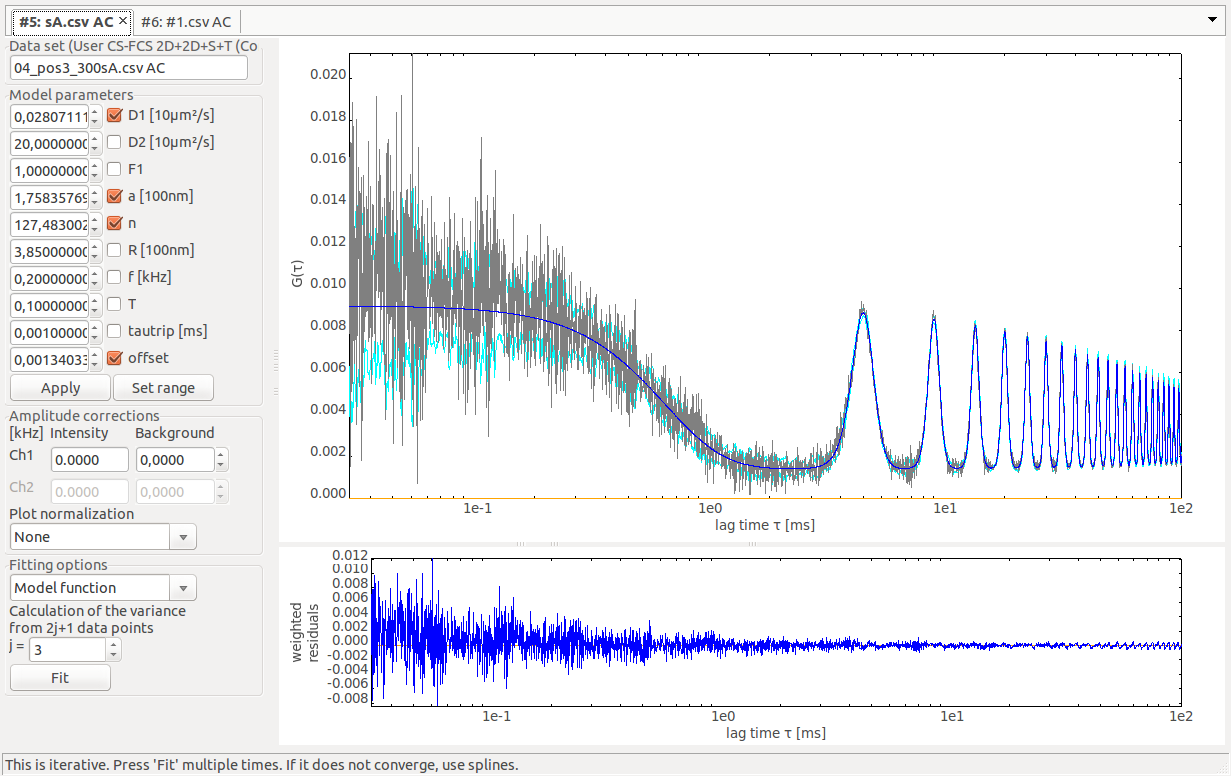
\includegraphics[width=\linewidth]{PyCorrFit_Screenshot_CSFCS.png}
 \mycaption{user interface with external model function}{cSFCS curve of DiO diffusing in a reconstituted lipid bilayer on glass support. Fitting yields a diffusion coefficient of \SI{0.28}{\mu m^2s^{-1}} ($F1=1$, so only one component is fitted). The source code of the external model function for this fit is shown in \hyref{Figure}{fig:csfcs}.\label{fig:csfcsplot}}
\end{figure}

\vspace{1em}
\subsubsection{Total internal reflection FCS (TIR-FCS)}
\label{sec:theor.exten.total}
TIR-FCS was developed to measure transient ligand binding events to receptors in the membrane \cite{Thompson2007}. In contrast to scanning FCS, the detection volume is fixed. However, the geometry is confined to the surface showing an exponential decay of the evanescent field along $z$, whereas the lateral boundaries imposed in $xy$ by a pinhole in the detection path. The situation is notoriously difficult to model and different solutions have been proposed.

\paragraph{TIR-FCS with Gaussian-shaped lateral detection volume.}
The detection volume is axially confined by an evanescent field and has an effective size of
\begin{align}
V = \pi R_0^2 d_\mathrm{eva}
\end{align} 
where $R_0$ is the lateral extent of the detection volume and $d_\mathrm{eva}$ is the evanescent field depth\footnote{Where the field has decayed to $1/e$}. From the concentration $C$, the effective number of particles is $n = CV$.
The decay constant $\kappa$ is the inverse of the depth $d_\mathrm{eva}$ :
\begin{align}
d_\mathrm{eva} = \frac{1}{\kappa}
\end{align} 

\paragraph{TIR-FCS with a square-shaped lateral detection volume.}
The detection volume is axially confined by an evanescent field of depth $d_\mathrm{eva} = 1 / \kappa$.
The lateral detection area is a convolution of the point spread function of the microscope of size $\sigma$,
\begin{align}
\sigma = \sigma_0  \frac{\lambda}{\mathit{NA}},
\end{align} 
with a square of side length $a$.


\subsection{Fitting}
\label{sec:theor.nonle}
One can define a distance $d(G,H)$ between two discrete functions $G$ and $H$ with the discrete domain of definition $\tau_1 \dots \tau_n$ as the sum of squares:
\begin{equation}
d(G,H) = \sum_{i=1}^n \left[ G(\tau_i) - H(\tau_i) \right]^2
\end{equation}
The least-squares method minimizes this distance between the model function $G$ and the experimental values $H$ by modifying $k$ additional fitting parameters $\alpha_1, \dots, \alpha_k$:
\begin{equation}
\chi^2 = \min_{\alpha_1, \dots, \alpha_k} \sum_{i=1}^n \left[ G(\tau_i,\alpha_1, \dots, \alpha_k) - H(\tau_i) \right]^2
\end{equation}
The minimum distance $\chi^2$ is used to characterize the success of a fit. Note, that if the number of fitting parameters $k$ becomes too large, multiple values for $\chi^2$ can be found, depending on the starting values of the $k$ parameters.


\subsubsection{Weighted fitting}
\label{sec:theor.weigh}
In certain cases, it is useful to perform weighted fitting with a known variance $\sigma_i^2$ at the data points $\tau_i$. In \textit{PyCorrFit}, weighted fitting is implemented as follows:
\begin{equation}
\chi^2_\mathrm{weighted} = \min_{\alpha_1, \dots, \alpha_k} \sum_{i=1}^n  \frac{\left[ G(\tau_i,\alpha_1, \dots, \alpha_k) - H(\tau_i) \right]^2}{\sigma_i^2}
\end{equation}

Besides importing the variance alongside experimental data, \textit{PyCorrFit} is able to estimate the variance from the experimental data via several different approaches. A recommended approach is averaging over several curves. Other approaches such as estimation of the variance from spline fits or from the model function (see \hyref{Section}{sec:intro.graph}) cannot be considered unbiased. 
Note that when performing global fits (see \hyref{Section}{sec:menub.tools.globa}), different types of weights for different correlation curves can strongly influence the result of the fit. Especially mixing curves with and without weights will most likely result in unphysical fits.

\subsubsection{Displayed $\chi^2$ values}
The displayed value of $\chi^2$ is defined by the type of the performed fit. This value is commonly normalized by the degrees of freedom $\nu = N - n - 1$, where $N$ is the number of observations (data points) and $n$ is the number of fitting parameters.
\begin{itemize}

\item \textbf{reduced expected sum of squares}: This value is used when there is no variance available for plot normalization.
\begin{equation}
\chi^2_\mathrm{red,exp} = \frac{1}{\nu}\sum_{i=1}^n  \frac{\left[ G(\tau_i,\alpha_\mathrm{min}) - H(\tau_i) \right]^2}{G(\tau_i,\alpha_\mathrm{min})}
\end{equation}

\item \textbf{reduced weighted sum of squares}: This  value is used when the fit was performed with variances $\sigma^2$.
\begin{equation}
\chi^2_\mathrm{red,weight} = \frac{1}{\nu}\sum_{i=1}^n  \frac{\left[ G(\tau_i,\alpha_\mathrm{min}) - H(\tau_i) \right]^2}{\sigma^2}
\end{equation}

\item \textbf{reduced global sum of squares}: This  value is used for global fits. The weights are computed identically to the situation with reduced weights, except that the variance $\sigma_\textrm{glob}^2$ may result in non-physical weighting (hence the emphasis on global).
\begin{equation}
\chi^2_\mathrm{red,weight} = \frac{1}{\nu}\sum_{i=1}^n  \frac{\left[ G(\tau_i,\alpha_\mathrm{min}) - H(\tau_i) \right]^2}{\sigma_\textrm{glob}^2}
\end{equation}

\end{itemize}


\subsubsection{Algorithms}
\label{sec:theor.alg}
\textit{PyCorrFit} uses the non-linear least-squares fitting capabilities from \texttt{scipy.optimize}. This package contains several algorithms to minimize the sum of the squares. 
PyCorrFit can utilize several algorithms to perform this minimization. The descriptions of the algorithms listed here are partly copied from the scipy documentation at \url{http://docs.scipy.org/doc/scipy/reference/optimize.html}. 
\begin{itemize}
\item The \textbf{BFGS} method uses the quasi-Newton method of Broyden, Fletcher, Goldfarb, and Shanno (BFGS) \cite{Nocedal2006} (pp. 136). It uses the first derivatives only. BFGS has proven good performance even for non-smooth optimizations.
\item The \textbf{Levenberg-Marquardt} algorithm \cite{Levenberg1944} uses the first derivatives and combines the Gauss–Newton algorithm with a trust region approach. It is very robust compared to other algorithms and it is very popular in curve-fitting. \textit{PyCorrFit} uses this algorithm by default. If this algorithm is used, \textit{PyCorrFit} can estimate an error of the fit parameters using the covariance matrix.
\item The \textbf{Nelder-Mead} method uses the Simplex algorithm \cite{Nelder1965,Wright1996}. This algorithm has been successful in many applications but other algorithms using the first and/or second derivatives information might be preferred for their better performances and robustness in general.
\item The method \textbf{Powell} is a modification of Powell's method \cite{Powell1964, Press} which is a conjugate direction method. It performs sequential one-dimensional minimizations along each vector of the directions set, which is updated at each iteration of the main minimization loop. The function need not be differentiable, and no derivatives are taken.
\item \textbf{Sequential Linear Squares Programming}  inherently accepts boundaries and thus might behave better than other algorithms for problems with  bounded parameters.
\end{itemize}

\subsection{Included model functions}
This is an overview of all the model functions that are currently\footnote{\today} implemented in PyCorrFit. To each model a unique model ID is assigned by PyCorrFit. The following information is also accessible from within PyCorrFit using the \textbf{Page info} tool.

\subsubsection{Confocal FCS}
The confocal detection volume with the structural parameter 
\begin{align}
\mathit{SP}= \frac{z_0}{r_0}
\end{align}
has an effective size of
\begin{align}
V = \pi^{3/2} r_0^2 z_0
\end{align}
where $r_0$ is its lateral and $z_0$ its axial (in case of 3D diffusion) extension. Thus, the effective number of particles is defined as
\begin{align}
N = C V
\end{align}
with the concentration $C$ given implicitly in the model functions.
The diffusion coefficient is calculated from the diffusion time $\tau_\mathrm{diff}$ using
\begin{align}
D = \frac{1}{4 \tau_\mathrm{diff}} \left( \frac{z_0}{\mathit{SP}} \right)^2 = \frac{r_0^2}{4 \tau_\mathrm{diff}}.
\end{align}
The parameters in the equation above need to be calibrated to obtain the diffusion coefficient. Usually a reference dye with a known diffusion coefficient is used to determine the lateral extension of the detection volume $r_0$ with a fixed structural parameter of e.g. $\mathit{SP}=4$.\\
\vspace{2em}


% 2D diffusion
\noindent \begin{tabular}{lp{.7\textwidth}}
Name & \textbf{2D (Gauß)} \\ 
ID & \textbf{6001} \\ 
Descr. &  Two-dimensional diffusion with a Gaussian laser profile. \\ 
\end{tabular}
\begin{align}
G(\tau) = A_0 + \frac{1}{N} \frac{1}{(1+\tau/\tau_\mathrm{diff}) )}
\end{align} 
\begin{center}
\begin{tabular}{ll}
$A_0$ & Offset \\ 
$N$ & Effective number of particles in confocal area \\ 
$\tau_\mathrm{diff}$ &   Characteristic residence time in confocal area \\
\end{tabular} \\
\end{center}
\vspace{2em}


% 2D diffusion + triplett
\noindent \begin{tabular}{lp{.7\textwidth}}
Name & \textbf{2D+T (Gauß)} \\ 
ID & \textbf{6002} \\ 
Descr. &  Two-dimensional diffusion with a Gaussian laser profile, including a triplet component. \\ 
\end{tabular}
\begin{align}
G(\tau) = A_0 + \frac{1}{N} \frac{1}{(1+\tau/\tau_\mathrm{diff}))}  \left(1 + \frac{T e^{-\tau/\tau_\mathrm{trip}}}{1-T}  \right)
\end{align} 
\begin{center}
\begin{tabular}{ll}
$A_0$ & Offset \\ 
$N$ & Effective number of particles in confocal area \\ 
$\tau_\mathrm{diff}$ &  Characteristic residence time in confocal area \\ 
$T$ &  Fraction of particles in triplet (non-fluorescent) state\\ 
$\tau_\mathrm{trip}$ &  Characteristic residence time in triplet state \\ 
\end{tabular}
\end{center}
\vspace{2em}


% 3D diffusion
\noindent \begin{tabular}{lp{.7\textwidth}}
Name & \textbf{3D (Gauß)} \\ 
ID & \textbf{6012} \\ 
Descr. &  Three-dimensional free diffusion with a Gaussian laser profile (eliptical). \\ 
\end{tabular}
\begin{align}
G(\tau) = A_0 + \frac{1}{N} \frac{1}{(1+\tau/\tau_\mathrm{diff}))} \frac{1}{\sqrt{1+\tau/(\mathit{SP}^2 \tau_\mathrm{diff})}}
\end{align} 
\begin{center}
\begin{tabular}{ll}
$A_0$ & Offset \\ 
$N$ & Effective number of particles in confocal volume \\ 
$\tau_\mathrm{diff}$ &  Characteristic residence time in confocal volume \\ 
$\mathit{SP}$ & Structural parameter, describes elongation of the confocal volume \\
\end{tabular}
\end{center}
\vspace{2em}


% 3D diffusion + triplet
\noindent \begin{tabular}{lp{.7\textwidth}}
Name & \textbf{3D+T (Gauß)} \\ 
ID & \textbf{6011} \\ 
Descr. &  Three-dimensional free diffusion with a Gaussian laser profile (eliptical), including a triplet component. \\ 
\end{tabular}
\begin{align}
G(\tau) = A_0 + \frac{1}{N} \frac{1}{(1+\tau/\tau_\mathrm{diff}))} \frac{1}{\sqrt{1+\tau/(\mathit{SP}^2 \tau_\mathrm{diff})}} \left(1 + \frac{T e^{-\tau/\tau_\mathrm{trip}}}{1-T}  \right)
\end{align} 
\begin{center}
\begin{tabular}{ll}
$A_0$ & Offset \\ 
$N$ & Effective number of particles in confocal volume \\ 
$\tau_\mathrm{diff}$ &  Characteristic residence time in confocal volume \\ 
$\mathit{SP}$ & Structural parameter, describes elongation of the confocal volume \\
$T$ &  Fraction of particles in triplet (non-fluorescent) state\\ 
$\tau_\mathrm{trip}$ &  Characteristic residence time in triplet \\
\end{tabular}
\end{center}
\vspace{2em}


% 2D+2D diffusion + triplett
\noindent \begin{tabular}{lp{.7\textwidth}}
Name & \textbf{2D+2D+T (Gauß)} \\ 
ID & \textbf{6031} \\ 
Descr. &  Two-component, two-dimensional diffusion with a Gaussian laser profile, including a triplet component. \\ 
\end{tabular}
\begin{align}
G(\tau) = A_0 + \frac{1}{N (F + \alpha (1-F))²} \left[ \frac{F}{1+\tau/\tau_1} + \alpha^2 \frac{1-F}{ 1+\tau/\tau_2 } \right] \left(1 + \frac{T e^{-\tau/\tau_\mathrm{trip}}}{1-T}  \right) 
\end{align} 
\begin{center}
\begin{tabular}{ll}
$A_0$ & Offset \\ 
$N$ & Effective number of particles in confocal area ($N = N_1+N_2$) \\ 
$\tau_1$ &  Diffusion time of particle species 1 \\ 
$\tau_2$ &  Diffusion time of particle species 2 \\ 
$F$ & Fraction of molecules of species 1 ($N_1 = F N$) \\
$\alpha$ & Relative molecular brightness of particles 1 and 2 ($ \alpha = q_2/q_1$) \\
$T$ &  Fraction of particles in triplet (non-fluorescent) state\\ 
$\tau_\mathrm{trip}$ &  Characteristic residence time in triplet state \\ 
\end{tabular}
\end{center}
\vspace{2em}


% 3D+2D diffusion + triplett
\noindent \begin{tabular}{lp{.7\textwidth}}
Name & \textbf{3D+2D+T (Gauß)} \\ 
ID & \textbf{6032} \\ 
Descr. &  Two-component, two- and three-dimensional diffusion with a Gaussian laser profile, including a triplet component. \\ 
\end{tabular}
\begin{align}
G(\tau) = A_0 + \frac{1}{N (1 - F + \alpha F)²} \left[ \frac{1-F}{1+\tau/\tau_\mathrm{2D}} + \frac{ \alpha^2 F}{ 1+\tau/\tau_\mathrm{3D} } \frac{1}{\sqrt{1+\tau/(\mathit{SP}^2 \tau_\mathrm{3D})}} \right] \left(1 + \frac{T e^{-\tau/\tau_\mathrm{trip}}}{1-T}  \right) 
\end{align} 
\begin{center}
\begin{tabular}{ll}
$A_0$ & Offset \\ 
$N$ & Effective number of particles in confocal volume ($N = N_\mathrm{2D}+N_\mathrm{3D}$) \\ 
$\tau_\mathrm{2D}$ &  Diffusion time of surface bound particles \\ 
$\tau_\mathrm{3D}$ &  Diffusion time of freely diffusing particles \\ 
$F$ & Fraction of molecules of the freely diffusing species ($N_\mathrm{3D} = F N$) \\
$\alpha$ & Relative molecular brightness of particle species ($ \alpha = q_\mathrm{3D}/q_\mathrm{2D}$) \\
$\mathit{SP}$ & Structural parameter, describes elongation of the confocal volume \\
$T$ &  Fraction of particles in triplet (non-fluorescent) state\\ 
$\tau_\mathrm{trip}$ &  Characteristic residence time in triplet state \\ 
\end{tabular}
\end{center}
\vspace{2em}


% 3D+3D diffusion + triplett
\noindent \begin{tabular}{lp{.7\textwidth}}
Name & \textbf{3D+3D+T (Gauß)} \\ 
ID & \textbf{6030} \\ 
Descr. &  Two-component three-dimensional free diffusion with a Gaussian laser profile, including a triplet component. \\ 
\end{tabular}
\begin{align}
G(\tau) &= A_0 + \frac{1}{N (F + \alpha (1-F))²}  \left(1 + \frac{T e^{-\tau/\tau_\mathrm{trip}}}{1-T}  \right)  \times \\
\notag &\times  \left[ \frac{F}{1+\tau/\tau_1}  \frac{1}{\sqrt{1+\tau/(\mathit{SP}^2 \tau_1)}} + \alpha^2 \frac{1-F}{ 1+\tau/\tau_2 }  \frac{1}{\sqrt{1+\tau/(\mathit{SP}^2 \tau_2)}} \right]
\end{align} 
\begin{center}
\begin{tabular}{ll}
$A_0$ & Offset \\ 
$N$ & Effective number of particles in confocal volume ($N = N_1+N_2$) \\ 
$\tau_1$ &  Diffusion time of particle species 1 \\ 
$\tau_2$ &  Diffusion time of particle species 2 \\ 
$F$ & Fraction of molecules of species 1 ($N_1 = F N$) \\
$\alpha$ & Relative molecular brightness of particles 1 and 2 ($ \alpha = q_2/q_1$) \\
$\mathit{SP}$ & Structural parameter, describes elongation of the confocal volume \\
$T$ &  Fraction of particles in triplet (non-fluorescent) state\\ 
$\tau_\mathrm{trip}$ &  Characteristic residence time in triplet state \\ 
\end{tabular}
\end{center}
\vspace{2em}



\subsubsection{Confocal TIR-FCS}
The detection volume is axially confined by an evanescent field and has an effective size of
\begin{align}
V = \pi R_0^2 d_\mathrm{eva}
\end{align} 
where $R_0$ is the lateral extent of the detection volume and $d_\mathrm{eva}$ is the evanescent field depth. From the concentration $C$, the effective number of particles is $N=CV$.
The decay constant $\kappa$ is the inverse of the depth $d_\mathrm{eva}$ :
\begin{align}
d_\mathrm{eva} = \frac{1}{\kappa}
\end{align} 
The equations below make use of the Faddeeva function (complex error function)\footnote{In user-defined model functions, the Faddeeva function is accessible through \texttt{wofz()}. For convenience, the function \texttt{wixi()} can be used which only takes $\xi$ as an argument and the imaginary $i$ can be omitted.}:
\begin{align}
w(i\xi) &= e^{\xi^2} \mathrm{erfc}(\xi) \\
\notag &= e^{\xi^2} \cdot  \frac{2}{\sqrt{\pi}} \int_\xi^\infty \mathrm{e}^{-\alpha^2} \mathrm{d\alpha} \label{eq:faddeeva}
\end{align} 
The lateral detection area has the same shape as in confocal FCS. Thus, correlation functions for two-dimensional diffusion of the confocal case apply and are not mentioned here. \\
\vspace{2em}


% 3D diffusion (Gauß/exp)
\noindent \begin{tabular}{lp{.7\textwidth}}
Name & \textbf{3D (Gauß/exp)} \\ 
ID & \textbf{6013} \\ 
Descr. &  Three-dimensional free diffusion with a Gaussian lateral detection profile and an exponentially decaying profile in axial direction. \\ 
\end{tabular}
\begin{align}
G(\tau) = \frac{1}{C}  \frac{ \kappa^2}{ \pi (R_0^2 +4D\tau)}
 \left( \sqrt{\frac{D \tau}{\pi}} + \frac{1 - 2 D \tau \kappa^2}{2 \kappa}  w\left(i \sqrt{D \tau} \kappa\right) \right)
\end{align} 
\begin{center}
\begin{tabular}{ll}
$C$ & Particle concentration in confocal volume \\ 
$\kappa$ &  Evanescent decay constant ($\kappa = 1/d_\mathrm{eva}$)\\ 
$R_0$ & Lateral extent of the detection volume \\
$D$ & Diffusion coefficient  \\
\end{tabular}
\end{center}
\vspace{2em}


% 2D+3D+T diffusion (Gauß/exp)
\noindent \begin{tabular}{lp{.7\textwidth}}
Name & \textbf{3D+2D+T (Gauß/exp)} \\ 
ID & \textbf{6033} \\ 
Descr. &  Two-component, two- and three-dimensional diffusion with a Gaussian lateral detection profile and an exponentially decaying profile in axial direction, including a triplet component. \\ 
\end{tabular}
\begin{align}
G(\tau) &= A_0 + \frac{1}{N (1-F + \alpha F)^2} \left(1 + \frac{T e^{-\tau/\tau_\mathrm{trip}}}{1-T}  \right)  \times \\
& \notag \times  \left[
\frac{1-F}{1+ 4 D_\mathrm{2D} \tau/R_0^2} + 
\frac{\alpha^2 F \kappa}{1+ 4 D_\mathrm{3D} \tau/R_0^2} 
\left( \sqrt{\frac{D_\mathrm{3D} \tau}{\pi}} + \frac{1 - 2 D_\mathrm{3D} \tau \kappa^2}{2 \kappa}  w\left(i \sqrt{D_\mathrm{3D} \tau} \kappa\right) \right) \right]
\end{align} 
\begin{center}
\begin{tabular}{ll}
$A_0$ & Offset \\ 
$N$ & Effective number of particles in confocal volume ($N = N_\mathrm{2D}+N_\mathrm{3D}$) \\ 
$\kappa$ &  Evanescent decay constant ($\kappa = 1/d_\mathrm{eva}$)\\ 
$D_\mathrm{2D}$ &  Diffusion coefficient of surface bound particles \\ 
$D_\mathrm{3D}$ &  Diffusion coefficient of freely diffusing particles \\ 
$F$ & Fraction of molecules of the freely diffusing species ($N_\mathrm{3D} = F N$) \\
$\alpha$ & Relative molecular brightness of particle species ($ \alpha = q_\mathrm{3D}/q_\mathrm{2D}$) \\
$R_0$ & Lateral extent of the detection volume \\
$T$ &  Fraction of particles in triplet (non-fluorescent) state\\ 
$\tau_\mathrm{trip}$ &  Characteristic residence time in triplet state \\ 
\end{tabular}
\end{center}
\vspace{2em}




\subsubsection{TIR-FCS with a square shaped lateral detection volume}

\section{Troubleshooting}
If you are having problems with PyCorrFit, you might find the solution in the frequently asked questions\footnote{\url{https://github.com/paulmueller/PyCorrFit/wiki/Frequently-Asked-Questions-\%28FAQ\%29}} or on other pages in the \textit{PyCorrFit} 
wiki\footnote{\url{https://github.com/paulmueller/PyCorrFit/wiki}}.
There you will also find instructions on how to contact us to file a bug or to request a feature.
